%
% Source available at https://github.com/bkaluza/PhDthesis
%
\documentclass[twoside,11pt]{MPSthesis}

%------------------------------------------------------------------
% Information for the title page
%

\author{Name Surname}	% Name and Surname of the Author

\title{THESIS TITLE IN ENGLISH}	% Title in English

\naslov{NASLOV NALOGE V SLOVEN{\v S}{\v C}INI}	% Title in Slovene 


\month{Month}
\year{2013} 
\version{}	% optional (should be empty in the final version)


\supervisor{title Name Surname}	% Supervisor: Name and Surname with the title
\cosupervisor{title Name Surname}	% Co-Supervisor: Name and Surname with the title

\supervisorlong{\supervisor, Jo\v{z}ef Stefan Institute, Ljubljana, Slovenia}
\cosupervisorlong{\cosupervisor, Jo\v{z}ef Stefan Institute, Ljubljana, Slovenia}

\evaluationBoardMember{title Name Surname}
\evaluationBoardMemberAffiliation{Affiliation}

\evaluationBoardChairman{title Name Surname}
\evaluationBoardChairmanAffiliation{Affiliation}

\evaluationBoardMembers{title Name Surname}
\evaluationBoardMemberAffiliations{Affiliation}



%------------------------------------------------------------------
% custom definitions and shortcuts
%



%===================================================================
% Document structure
%
\begin{document}

%---------------------------------------------------------------------
% Front pages
%

% <--- DO NOT EDIT START -->
\frontmatter
\makepreamble
\maketitle 

\cleardoublepage
\begin{dedication} %this creates the heading for the dedication page

% No full stop
This is dedication page...


\end{dedication}



\newpage \thispagestyle{empty}

\cleardoublepage
\fancyhead{}
\fancyfoot{}
\fancyhead[RO]{\footnotesize \thepage}
\fancyhead[LO]{}
\fancyhead[LE]{\footnotesize \thepage}
\fancyhead[RE]{\footnotesize {Contents}}
\renewcommand{\contentsname}{\vspace{-2.4cm} \Large Contents \vspace{1.5cm}}
\tableofcontents
\newpage \thispagestyle{empty}

\cleardoublepage
\include{frontmatter/abstract}
\newpage \thispagestyle{empty}

\cleardoublepage
\include{frontmatter/povzetek}
\newpage \thispagestyle{empty}

\cleardoublepage
\include{frontmatter/abbreviations}
\newpage \thispagestyle{empty}

\mainmatter
\mychapterstyle
% <--- DO NOT EDIT STOP -->

%---------------------------------------------------------------------
% Chapters
%

\chapter{Introduction}

This Chapter explains how to provide citations, publications related to the dissertation and abbreviations throughout the thesis. 

%The thesis starts with a short overview of the area, positioning of the thesis, the main goals and the hypothesis of the thesis. 
\section{Citations}
In order to use the correct bibliography style, the bibliography style \textit{mps4$\_$5} is included in the main file \textit{thesis.tex}. Several examples for citations are provided in continuation.

\begin{enumerate}
	\item Article citation: \cite{Saaty2003a}, \citep{Saaty2003}
	\item Web page citation: \citep{TheEconomist2010}
	\item Author citation: \cite{Zopounidis2006}
	\item Book citation: \citep{BohanecDEXi2011}
	\item Conference article citation: \citep{Baracskai2003}
	\item Several citations: 
	\subitem \citep{BohanecDEXi2011, Burstein2008, Power2002}
	\subitem  \citep{Skinner1999, Ronald} 
	\subitem   \citep{Triantaphyllou, French, Bouyssou2006}
	\subitem \citep{Figueira2005}
	\subitem \citep{Jacquet-Lagreze1982} 
	\subitem \citep{Saaty2008}
	\subitem \citep{Moshkovich1995}
	\subitem \citep{GrecoRSMCDA}
	\subitem \citep{Adam2008, Figueira2005, Bouyssou2006}
	\subitem \citep{Menzies2006, Saaty2008, Zadeh1975, Guo2009, Barron1996} 
\end{enumerate}

\section{Publications related to the dissertation}
Publications related to the dissertation should be entered in  \textit{myPublication.bib} file. In order to enter them in Chapter~\ref{sec:publications}, one should cite (include) them in the file \textit{my$\_$publications.tex}.

In order a publication to appear in the chapter \emph{Publications related to the dissertation}, after changing the file \textit{my$\_$publications.tex}, one has to run \textit{bibtex bu.aux} for all bu*.aux files (bu1.aux, bu2.aux etc.). After compiling, the references to the publications will appear.


\section{Abbreviations}
The first occurrence of an abbreviation has to be followed with its long explanation. See the examples below for different types of abbreviations.

To add a new abbreviation, in the file \emph{abbreviation.txt} use the following command:
\begin{verbatim} 
   \newacronym\<label>}{<abbrv>}{<full>}
\end{verbatim}

In order to make the abbreviations appear in the list of abbreviations, the following procedure should be applied:
\begin{enumerate}
	\item {Apply latex compile twice (from the editor or in command line by using the command latex thesis.txt}
	\item{Run the following two commands in command line:}
		\subitem {makeindex -s thesis.ist -t thesis.alg -o thesis.acr thesis.acn}
		\subitem {makeindex -s thesis.ist -t thesis.glg -o thesis.gls thesis.glo}
\end{enumerate}
%or simply run sh mkGloss.sh in the command line.

Afterwards the latex compile will include the list of abbreviations. Any content changes in the file \emph{abbreviation.txt}, require repeating the above procedure in order for changes to take effect.

The first occurrence of an abbreviation has to be followed with its long explanation. Several examples of usage of long abbreviations are given in continuation.

\begin{itemize}
	%\item Adding an abbreviation and a citation: \gls{qq} \citep{BohanecBook}. \gls{qq} is an abbreviation that has been already included. 
	%\item \Gls{FNAC} is an abbreviation at the beginning of the sentence.
	%\item Adding a new abbreviation in text for \gls{icf}.
	%\item Usage of the long plural form of the acronym: \acrlongpl{icf}. 
	%\item Usage of the long singular form of the acronym: \acrlong{icf}.
	%\item Usage of the short plural form of the abbreviation: \acrshortpl{icf}. 
	%\item Usage of the short singular form of the abbreviation: \acrshort{icf}.
	\item test
\end{itemize}


\section{Contribution}

This is a new section.


\section{Organization of the thesis}

This is a new section.



This Chapter explains how to provide Definitions, Theorems, Lemmas and Algorithms in the thesis.

\section{Definitions, Theorems, Lemmas}

%\begin{definition}
%		This is definition.
%\end{definition}

%\begin{theorem}
%		This is theorem. 
%\end{theorem}

%\begin{lemma}
%		This is lemma. 
%\end{lemma}

\section{Algorithms}

This is an example of how to write an Algorithm by using the packages \textit{algorithm} and \textit{algorithmic}.

% \begin{algorithm} 
% \caption{Regression algorithm for FNAC structure and dependent variable in the $p$ position}
% \label{alg_2}
% 	\begin{algorithmic}[1]
% 		\State $v\gets 0.5$ 
% 		\State $q\gets 0.5$ \Comment{calculate median regression for $q=\frac{1}{2}$}
% 		\If {$p==n$}		\Comment{if regression variable is positioned last;  n is the number of random variables/attributes};
% 				\State $v\gets [1-u^{-\theta}+(qu^{1+\theta})^{-\frac{\theta}{1+\theta}}]^{-\frac{1}{\theta}}$ \Comment{calculate $v$}
% 		\Else
%     		\For{$j = 1 \to (n-p)$,  \\ (or $j = 1 \to (n-2)$, when p=1,2) } \Comment{if position of regression variable other than the last}
% 				\State $q\gets v$ \Comment{replace $q$ with the value of $v$}
% 				\State $v\gets [1-u^{-\theta}+(qu^{1+\theta})^{-\frac{\theta}{1+\theta}}]^{-\frac{1}{\theta}}$  \Comment{recalculate the new value of $v$}
% 				\State $i\gets i-1$ 
% 			\EndFor \Comment{$p$ is the output variable position}
% 			\State $q\gets v$ \Comment{replace $q$ with the value of $v$}
% 			\State $v\gets [1-u^{-\theta}+(qu^{1+\theta})^{-\frac{\theta}{1+\theta}}]^{-\frac{1}{\theta}}$  \Comment{recalculate $v$; if $p=1$, $u=u_2$; if $p=2$, $u=u_1$}
% \EndIf

% \State $u\gets F_1(x_1)$ \Comment{replace $u$ by $F_1(x_1)$}
% \State $v\gets F_2(x_2)$ \Comment{replace $v$ by $F_2(x_2)$}
		
% 	\end{algorithmic}
% 	\end{algorithm}


This Chapter provides examples of formatting Figures and Tables. 

\section{Formatting figures}
An example of how to format several drawings in one figure is provided on Figure~\ref{fig:QQ_different_weights}.
% \begin{figure}[!htb]
% \centering
% \subfloat[Caption of Figure - a]{
% 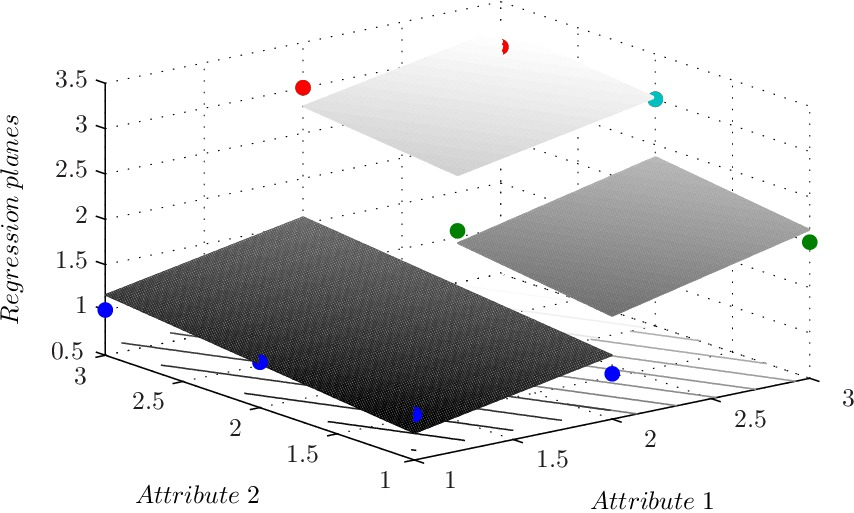
\includegraphics{./figures/chapter3/imga.jpg}
% \label{fig:QQ_ginibrei}
% }
% \\
% \subfloat[Caption of Figure - b]{
% 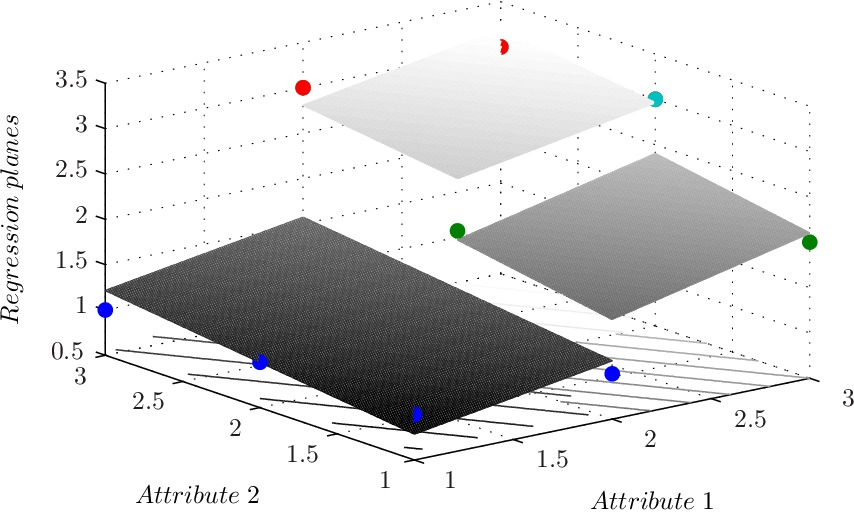
\includegraphics{./figures/chapter3/imgb.jpg}
% \label{fig:QQ_ginicov}
% }
% \quad
% \subfloat[Caption of Figure - c]{
% 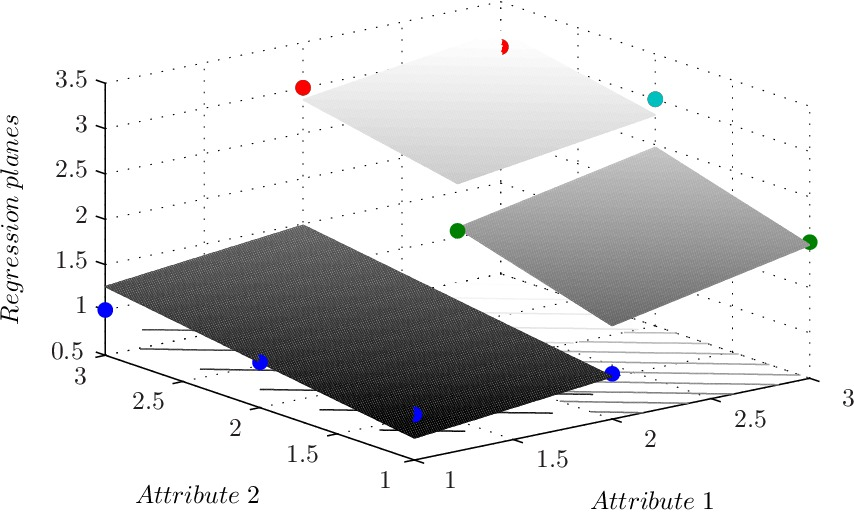
\includegraphics{./figures/chapter3/imgc.jpg}
% \label{fig:QQ_ginipop}
% }
% \caption{Caption of the Figure}
% \label{fig:QQ_different_weights}
% \end{figure}


\subsection{Subsection}
\label{sec:subsection}
This is an example of subsection.

\paragraph{This is a pragraph}
This is an example of a paragraph within the subsection~\ref{sec:subsection}.

\subsubsection{Subsubsection}
This is an example of subsubsection. The maximal depth of numbered subsections is 2.

\section{Formatting Tables}
An example of how to format a table is given in Table~\ref{tbl:QQqual}. Shadings are not a requirement.

\begin{table}[!ht]
\centering
\caption{Qualitatively described problem}
\begin{tabular}{cccc}
\toprule 
\textbf{No.} & ${{\mathbf {QA}}}_{{\mathbf 1}}$\textbf{} & ${{\mathbf {QA}}}_{{\mathbf 2}}$\textbf{} & 		\textbf{QC} \\
\midrule
1 & good & good  & good \\ 
2 & better & good & good \\ 
3 & good & better & good \\ 
4 & good & the best & good \\ 
\rowcolor[gray]{0.9} 5 & the best & good & better\\ 
\rowcolor[gray]{0.9} 6 & better & better & better \\ 
7 & the best & better & the best \\ 
8 & better & the best & the best \\ 
9 & the best & the best & the best \\ 
\bottomrule 
\end{tabular}
\label{tbl:QQqual}
\hspace{0.5cm}
\end{table}


%
% In order to color the first row cell/-s, \rowcolor[gray]{0.9} is used.
% The word 'gray' here denotes the grayscale color scheme, not the color grey and `0.9' denotes how dark the grey is.
%
% The xcolor package provides the necessary commands to produce tables with alternate row colors, when loaded with the table option.
% The command \rowcolors{<starting row>}{<odd color>}{<even color>} has to be specified right before the tabular environment starts.
%
% For footnotes to work inside of tables, apply minipage environment before entering tabular environment.

\newpage \thispagestyle{empty}

\include{chapters/chap2}
\newpage \thispagestyle{empty}

\include{chapters/chap3}
\newpage \thispagestyle{empty}

% Optional: make parts
%\part{Part 1}
%\label{part:myPart1}

%
% Include additional chapters here
%
%\include{chapters/my_chapter}
%\newpage \thispagestyle{empty}



%---------------------------------------------------------------------
% Endmatter
%

\chapter{Acknowledgements}
The research of the author was supported by Ad Futura Programme of the Slovene Human Resources and Scholarship Fund. I would also like to acknowledge the support of the Slovenian Research Agency through Research Programme XY-ZZVR.  






\newpage \thispagestyle{empty}

\bibliographystyle{MPSPhDBib}                      % bibliography style with names and years
\renewcommand{\bibname}{References}         % changes default name Bibliography to References
\cite{*}
\bibliography{references,myPublications} % References 


\cleardoublepage
\fancyhead{}
\fancyfoot{}
\fancyhead[RO]{\footnotesize \thepage}

\fancyhead[LE]{\footnotesize \thepage}
\fancyhead[RE]{\footnotesize {List of Figures}}
\addcontentsline{toc}{chapter}{List of Figures}
\renewcommand\listfigurename{\vspace{-2.4cm} \Large List of Figures \vspace{1.5cm}}
\listoffigures


\cleardoublepage
\fancyhead{}
\fancyfoot{}
\fancyhead[RO]{\footnotesize \thepage}
\fancyhead[LO]{}
\fancyhead[LE]{\footnotesize \thepage}
\fancyhead[RE]{\footnotesize {List of Tables}}
\addcontentsline{toc}{chapter}{List of Tables}
\renewcommand\listtablename{\vspace{-2.4cm} \Large List of Tables \vspace{1.5cm}}
\listoftables

\cleardoublepage
\fancyhead{}
\fancyfoot{}
\fancyhead[RO]{\footnotesize \thepage}
\fancyhead[LO]{}
\fancyhead[LE]{\footnotesize \thepage}
\fancyhead[RE]{\footnotesize {List of Algorithms}}
\addcontentsline{toc}{chapter}{List of Algorithms}
\listof{myalgorithm}{\vspace{-2.4cm} \Large List of Algorithms \vspace{1.5cm}}


%---------------------------------------------------------------------
% Appendencies
%
\appendix
\part*{Appendices}
\label{part:appendices}

\chapter*{\vspace{-2.3cm} \Large Appendix A: Bibliography \vspace{1.7cm}}
\addcontentsline{toc}{chapter}{Appendix A: Bibliography}
\label{chap:pub}

\fancyhead[LO]{}
\fancyhead[RE]{Appendix A: Bibliography}

\section*{Publications related to the dissertation}
%\label{sec:publications}
%\vspace{-.7cm}

\subsection*{1.01 Original scientific article}
\begin{itemize}
	\item \bibentry{BiljanaIJDSST2012}
	\item \bibentry{BiljanaDSS2012} 
	\item \bibentry{BiljanaOR2011} 
\end{itemize}


\subsection*{1.08 Published scientific conference contribution}
\begin{itemize}
	\item \bibentry{BiljanaIJDSST2012}
	\item \bibentry{BiljanaDSS2012} 
	\item \bibentry{BiljanaOR2011} 
\end{itemize}


\newpage \thispagestyle{empty}

\chapter*{\vspace{-2.3cm} \Large Appendix B: Biography \vspace{1.7cm}}
\addcontentsline{toc}{chapter}{Appendix B: Biography}
\label{chap:pub}

\fancyhead[LO]{}
\fancyhead[RE]{Appendix B: Biography}

%\chapter{Publications related to the dissertation}
%\label{sec:publications}
%\vspace{-.7cm}

This is biography...

\newpage \thispagestyle{empty}


\end{document}
